\chapter{Towards a Citizen Science-Enabled Liquid Democracy Platform}
\label{ch:Approach}
In the previous chapter we provided a theoretical background for citizen science and liquid democracy, showing amongst other things that potential synergies between the two concepts exist.
Therefore, in this chapter we aim to lay the conceptual foundation for a citizen science-enabled liquid democracy platform.
To this end, we will start by deriving a list of criteria such a platform would need to fulfill in \ref{sec:Criteria} before we evaluate existing work based on compliance with these criteria in \ref{sec:RelatedWork}.
Finally, we will present a thorough conceptual sketch of a citizen science-enabled liquid democracy platform in \ref{sec:Conceptual_Approach}.

%nach 3.3
%Thus, this system consists of two core components: (1) a participatory system, which is scaffolding the other core component: (2) an interface allowing interested users to access the system’s data. (1) is describing the concept of liquid democracy and (2) the approach of citizen science.

\section{Criteria}
\label{sec:Criteria}
In this section we want to gather criteria for a \tracknshrink{CS}-enabled \tracknshrink{LD} platform in order to evaluate existing projects on the one hand, and to approach the conceptual design of such a system on the other hand. 
Since we can not enumerate all the possible \tracknshrink{CS} projects with \tracknshrink{LD} backgrounds, we do not think that it is feasible to design a one-fits-all platform.
On the other hand, the \tracknshrink{LD} functionalities of specific platforms can be assumed to not change from project to project.
Therefore, we arrange our criteria in two groups.
Criteria in the first group are directed towards a general \tracknshrink{LD} platform design that can be used in projects both with and without a \tracknshrink{CS} context.
Those in the second group are directed towards a \tracknshrink{CS}-enabling interface a \tracknshrink{LD} platform can implement in order to explicitly support the development of specific \tracknshrink{CS} projects on top of it.

Based on our work in \ref{sec:Liquid_Democracy}, we derive the core functionalities of a \tracknshrink{LD} platform as \textbf{(\tracknshrink{LD}1)} collaborative editing of propositions, \textbf{(\tracknshrink{LD}2)} secret and verifiable voting on propositions and \textbf{(\tracknshrink{LD}3)} secret and verifiable vote delegation.
From \textbf{(\tracknshrink{LD}2)} and \textbf{(\tracknshrink{LD}3)} we extract that votes and delegations should not be tampered with by a adversary party.
An effective way to prevent this is to require \textbf{(\tracknshrink{LD}4)} decentralized publication of votes and delegations.
We observe that participatory systems on the web tend to produce an overwhelming amount of data and that most modern platforms tackle this problem by content filtering algorithms, which we do not consider to be appropriate for a \tracknshrink{LD} platform due to the danger of censorship.
Rather, we would like to involve the user to actively filter propositions and therefore derive the fifth criterion for a \tracknshrink{LD} platform as \textbf{(\tracknshrink{LD}5)} active information filtering capabilities.
Furthermore, as each individual in a \tracknshrink{LD} has the right to create propositions, we acknowledge that adversary users could abuse this right to generate a lot of noise (so called spam) in the fashion of a DDoS attack\footnote{\url{https://en.wikipedia.org/wiki/Denial-of-service_attack\#Distributed_DoS}}. Therefore we derive \textbf{(\tracknshrink{LD}6)} implementation of spam prevention mechanisms.
Finally, we derive the last criterion for a \tracknshrink{LD} platform from the discussion in \ref{ssec:Integration_AccessibilityAnonymity} as \textbf{(\tracknshrink{LD}7)} protection of privacy.

We have seen in \ref{sec:Theory_CS} that we can categorize a citizen science project according to the degree of participation and its expected outcome.
Our approach allows the implementation of \tracknshrink{LD}-based \tracknshrink{CS} projects on all levels of Hakalays ladder of participation, since our \tracknshrink{CS}-enabling interface empowers citizen science communities to kickstart their own projects and formulate research questions without the help of professional scientists.
Note that specifically the separation of the \tracknshrink{LD} platform from the \tracknshrink{CS}-enabling interface means that communities could build their \tracknshrink{CS} projects either around existing instances of \tracknshrink{CS}-enabled \tracknshrink{LD} platforms or, if needed, set up their own instance.
The main issue to solve with this interface is the conflict between user privacy, in particular secret voting, and data transparency as layed out in \ref{ssec:Integration_AccessibilityAnonymity}.
For lower levels of participation a more restrictive data access policy could be enforced, while higher levels of participation with involvement of the citizen scientists in the data evaluation and possibly even in the definition of research questions require complete and transparent access to all of the platforms data such as propositions, delegation graphs, voting results etc.
In order to support the highest level of participation possible we see no other way than to trust in the citizen scientists self-responsibility, i.e. to partly relay control over the amount and kind of data shared to the users of the \tracknshrink{LD} platform.
However, since users are not expected to be well trained in privacy protection, the choices of users should not be too fine-grained and rather be envisioned as a number of pre-specified policies.
We therefore derive the additional criteria for a \tracknshrink{CS}-enabling interface as \textbf{(\tracknshrink{CS}1)} complete access to non-sensitive platform data, \textbf{(\tracknshrink{CS}2)} default restrictive access to sensitive platform data with guaranteed privacy protection and \textbf{(\tracknshrink{CS}3)} opt-in completely transparent access access to sensitive platform data without guaranteed privacy protection.

\section{Related Work}
\label{sec:RelatedWork}
  
In this section we will explore related projects, that are freely accessible, open source software (\tracknshrink{FOSS}) and which share our two main goals; That is a platform allowing---to some extent---to (1) participate in democratic processes and (2) to access the platform’s data. Therefore, we do not focus on projects that implement regular survey/polling features (e.g., \textit{LimeSurvey}\footnote{\url{https://www.limesurvey.org/}}), as this would be only a small subset of that platform.

Initially, when starting this work in 2017, we discovered some projects that met certain aspects of our main goals. Most of these projects, however, have been (officially) discontinued over time or have not been under active development (no commit for two years or more). Additionally, some of them were commercial projects or closed-source and thus not replicable or adaptable in any way. The website \textit{The Democracy Foundation}\footnote{\url{https://democracy.foundation/similar-projects/}} provides a list ranging from smaller projects to advanced governance platforms. Unfortunately, most of them are outdated as well or are not applicable to our scenario. Nonetheless, there were two potential candidates we took into consideration for building a prototype.

The first promising platform we looked into was \textit{LiquidFeedback}\footnote{\url{https://liquidfeedback.org/}}. It is developed by the \textit{Public Software Group}\footnote{\url{https://www.public-software-group.org/}} and was used by Berlin’s Pirate Party for inner-party decision-making processes. Although the source code is available at the developers’ website, we encountered two major drawbacks. For one, we had difficulties during the setup process\footnote{\url{http://www.public-software-group.org/mercurial/liquid_feedback_frontend/raw-file/tip/INSTALL.html}}, and since there is no developer support (and no official repository, or other public developer community) it is a cumbersome process. Despite being labeled open source it is in the interest of the developer to implement the platform as payed service. Additionally, due to the large usesage of the programming language Lua---where none of us had any prior experience---we decided to skip this project.

The other candidate is \textit{DemocracyOS}\footnote{\url{http://democracyos.org/}}, which is actively developed by Argentina’s Net Party (span. \textit{Partido de la Red}). This platform provides a modern tech stack (backend: MongoDB, frontend: React) and good developer support\footnote{Docs: \url{http://docs.democracyos.org/} GitHub: \url{https://github.com/DemocracyOS/democracyos}}. Unfortunately, the project is structured in an obscure manner; for example the developers decided against differentiating between \texttt{src} files and \texttt{lib} files, thus mixing React components with regular helper functions and other libraries in on big \texttt{lib} folder. Since there is no clear separation of view, logic and helper libraries this creates an entangled graph of dependencies.

Despite both platforms, especially the latter one, being promising tools, there is still one fundamental issue: As of 2019 there is no \tracknshrink{FOSS} platform that implemented the idea of vote delegation in any way, and does provide sufficient support to engage developers. Since developing our very own digital liquid democracy platform would be an enormous project, we shifted our focus towards developing a conceptual framework.



% Participedia is a meta website gathering data from other sites:
% \url{https://www.wissenschaftsmanagement.de/news/participedia-demokratie-staerken-durch-geteiltes-wissen-und-bielefelder-forscher-entwickeln}

% nVotes is a simple voting plattform this could also be done with normal survey platforms such as LimeSurvey, so this not taken into account

\section{Conceptual Design}
\label{sec:Conceptual_Approach}
In this section we will develop a conceptual overview of both a \tracknshrink{LD} platform and a \tracknshrink{CS}-enabling interface based on the criteria derived in \ref{sec:Criteria}.
This task will be approached methodically from three conceptual views: artifacts, user roles and processes.
We start by describing different artifacts that occur within a liquid democracy.
%Namely, these are propositions, the centerpiece of democratic discourse: propositions, their properties and lifecycle.
Then we describe the various roles users can take in the platform.
Having a clear view on both artifacts and user roles, we then discuss the core processes of a \tracknshrink{CS}-enabled \tracknshrink{LD} platform.
%Lastly, we elaborate the utility of notifications for a \tracknshrink{LD} platform and illustrate how the \tracknshrink{CS}-enabling interface exhibited by the platform can be used by citizen science projects.

\subsection{Artifacts}
\label{ssec:data_fragments}
%In this section, we will present the essential artifacts in a \tracknshrink{LD} platform.

\subsubsection{Propositions}
\label{sec:Model_Propositions}
The most important tool in a democracy to transform political positions and individual opinions into laws are propositions.
In the remainder of this work, by propositions we are referring to political proposals that motivate a change in legislation and enumerate a list of possible options for this particular change, which participants in a democracy can vote on.
Apart from a title, the propositions motivational text and a list of voting options, propositions possess additional metadata and dependency relationships to other artifacts in the platform.
Metadata is very important for the accessibility of the actual information content, for example through active filtering mechanisms as required by \textbf{(\tracknshrink{LD}5)}.
Amongst others, proposition metadata include proposition creator, time of creation and the political context(s) as well as the administrative unit a proposition belongs to.

By political contexts (from here on just named \textit{contexts}), we mean the categorial themes in which political topics are organized.
The context a proposition is associated with is a crucial piece of metadata in a \tracknshrink{LD} platform, as  clearly defined categories are important to make order of the ongoing topics and are essential to stay on top of things.
As with most categorial organization systems, broad, general contexts can be divided down to narrower, more specficic ones and thus form a taxonomy, which we will discuss in detail in~\ref{sec:Model_Contexts}.

As described in~\ref{sec:Model_Contexts}, issues belong to different, sometimes multiple contexts. In order to allow for the versatility demanded there, but recognizing that a principle context (at some level within the taxonomy) is the focus of a proposition, we decided to assign a primary context and an arbitrary number of secondary contexts to the proposition as part of its metadata. Since the primary context addresses the very core of the proposition, changing the primary context is not possible. These restrictions are lifted for secondary context. With this, we believe to have reached a good compromise between keeping the identity of a context intact, while allowing for large flexibility.

Propositions typically evolve over time which can be conceptualized as a succession of versioned snapshots.
To this end, a propositions state should be saved together with an increasing version number at either fixed time intervals or manually by the individuals involved with the editing.
Moreover, a propositions creation and its evolution should always be accompanied by a healthy discussion of the matter at hand between both individuals directly involved with the proposition editing and other individuals interested in expressing their political opinions.
These discussions contents and their metadata are discussed in the next section.

\subsubsection{Discussion Entries}
\label{ssec:Discussion_Entries}
Discussion entries are posts from users that can be attached to several other artifacts that allow discussion.
To allow an efficient evaluation of participants opinions on the direction of the discourse, discussion entries can be up- or downvoted by other users.
Additionally, the textual content of a discussion entry can carry hyperlinks to a selection of other artifacts that it references.
Examples of artifacts that should be referencable by hyperlinks in discussion entries are propositions, proposition change requests and discussion entries themselves.

\subsubsection{Proposition Change Requests}
\label{ssec:Proposition_Change_Requests}
As we discussed briefly in the previous section about propositions, a proposition will evolve over its life time which means that it will be edited.
We argue that only the original creator of the proposition, i.e. its owner, should be able to directly edit it in order to ensure its consistency and prevent malicious editing of propositions by individuals with different opinions.
It is therefore also a measure of minority protection.
Since it is desirable that edits to propositions are based on a discursive process involving multiple individuals as required by \textbf{(\tracknshrink{LD}1)}, we introduce proposition change requests, which are artifacts that carry the edited propositon text together with a linked discussion entry and a reference to the underlying proposition. 
These proposition change requests can then be accepted or rejected by the owner of the proposition.
In addition to up- or downvoting the linked discussion entry, users can explicitly express their conditional support of the proposition in case the proposition change request gets accepted or rejected.
This should help the responsible proposition owners to determine the value of specific change requests.
Proposition change requests should not be used to completely turn a propositions goal on its head.
For these cases there exists alternative propositions which will be discussed next.

\subsubsection{Alternative Propositions and Proposition Groups}
\label{ssec:AltProposition}
In most cases, politics are too complex to capture the endeavor of all individuals in one proposition that can be answered with a simple yes or no.
In order to provide means to depict political opinions more accurately, we introduce alternative propositions.
Alternative propositions have all the properties of normal propositions with the exception that the primary political context of an alternative proposition can not be different from those of the original proposition. This allows for large versatility of the proposition, while ensuring that both propositions address the same (political) context.
Additionally, alternative propositions carry a reference to the original proposition, effectively placing them in a common \emph{proposition group}.

\subsubsection{Context Taxonomy}
\label{sec:Model_Contexts}
While we earlier looked at contexts as metadata of propositions, in order to categorize propositions effectively, a context taxonomy must exist prior to proposition creation, which makes such a taxonomy an independent artifact.

Choosing a proper context taxonomy to categorize propositions is crucial for a \tracknshrink{LD} project as it is a sort of foundation for the work to follow.
On the one hand the contexts can help users to find votes they are interested in, which partly satisfies criteria \textbf{(\tracknshrink{LD}5)}.
Even more important, with contexts the political subject can also determine for which issues they want to vote for themselves and which topics they want to pass on to a person with more expertise in this field.
Taking for example a vote about the deforestation of the south of Germany; a proposition about this matter could fall into a context as environmental politics (or in a more fine-grained taxonomy in the context of forestry).
Imagining that someone is not that much of a specialist when it comes to environmental politics, they could delegate votes for all propositions on this subject to a political subject they trust and assume to be knowledgeable about this context. The example could also be assigned to a regional context (southern Germany, or more specifically the region concerned), allowing to discern regional interest (and the interest of the people affected by decisions in this context). These contexts are not mutually exclusive, and a proposition could be assigned to several (non-exclusive) contexts.
%Here the taxonomies not only determine if he gets the topic in his feed but it also could automatically be passed on to his relative.
%This highlights a second problem: how do we make sure that the votes are categorized properly?
%More about this later.
%First, we have to make sure to set up a fundamental category that covers a wide spectrum of the political issues existing.

In general, a taxonomy for \tracknshrink{LD} propositions should meet three elemental requirements.
First and foremost, the taxonomy must be exhaustive as we want to make sure that every occurring proposition is covered.
Secondly the categories need to be disjoint\footnote{With the exception of hierarchically dependent categories}, meaning that two categories shouldn't describe the same subject.
Additionally, the categories should be able to adapt and evolve as the political landscape as well changes with time.
A taxonomy that fulfills all requirements perfectly probably does not exist, but we tried to find one already existing system that met our requirements as best as possible.

An exception to the second criterion for a taxonomy (its disjoint status) are hierarchically dependent categories. While taxonomies in the strict sense don't exhibit meronomic (i.e. part-whole) relationships, in practice they often do. This is particularly the case with geographic categories (e.g. states or counties within a country and municipalities within a state), but it also concerns fields or topics of politics. In the example above, forestry could be seen as a sub-category of environmental (or  economic) politics, and can further be broken down in sub-contexts that address more specific issues. While connections to other areas exist (e.g. forestry being a part of economic or environmental politics, and forestry being connected to matters concerning groundwater, erosion, micro-climate, biodiversity, air quality and pollution as well as carbon (net) emission politics to mention just a few), relationships of sub- and super contexts allows for much flexibility and versatility of contexts. Complex connections between different categories on the same hierarchical level can be achieved with allowing to assign sub-categories to several super-categories\footnote{e.g. by forestry politics being part of environmental and economic politics or more fine-grained categories being sub-categories of forestry, biodiversity and groundwater politics}.

A well-known external source for document categorization is the Wikipedia taxonomy.
The corpus of the open encyclopedia is often used to build automatic categorization approaches or to improve the performance of existing models.
Its pure size and the fact that it is constantly updated are very good reasons for this.
However, upon manual investigation we observed that the political categories in Wikipedia describe fields of political science rather than general topics politics are coping with. 
Therefore, this taxonomy is unfortunately not useful for our goals.

Almost the complete opposite is true for the taxonomy of Stack Overflow Politics.
While the Wikipedia articles were almost purely about a scientific view on Politics, the branch of the well-known question and answer site Stack Overflow almost only consist of current topics discussed by the community.
The created tags are therefore more useful for characterizing political topics.
But as the issues discussed are tagged by the user posting the question, it often occurs that there are two tags describing the same field.
The poor data quality of the Stack taxonomy and the necessity for time-consuming clean-up made this data source rather unattractive.

As a more organized data source that still addresses political topics instead of subjects of political science, we chose the taxonomy that classify the topics discussed by the Bundestag.
For every new legislation period, the parliament puts together committees for different topics.
Even if the number and names of these committees have slightly changed over time, the content is more or less consistent over time.
The official website of the Bundestag groups protocols of the committees' meeting into 43 topics describing a wide range of political topics.
From family to energy the categories are clearly structured, exhaustive and disjoint, therefore covering two of our three requirements. Since it furthermore changes slightly over time, our third requirement is partly met as well.

Hence, we recommend to use this taxonomy as a starting point for newly created \tracknshrink{LD} platform instances.
We note that in order to meet our third requirement, the platform should possess mechanisms for the collaborative editing of the taxonomy which will be described in section~\ref{ssec:Context_Taxonomy_Evolution}.

\subsubsection{Delegation Graphs}
%Vote delegation is the process of transferring voting rights for a proposition or a context (or a number of them) to a delegate.
%Technically this means that the vote of the delegate is counted several times (once for the delegate as voting right holder and once for each delegation towards him).
%From a social perspective this means a transfer of trust from the delegator to the delegate in an area of trust, whether this may be established from expertise, sympathy or other reasons.
%As such, the delegation mechanism encompasses attracting support publicly (what would be campaigning for a vote as a candidate in the representative system), friendship, different trust-based mechanisms and much more; These social phenomenon however are not technically relevant for a \tracknshrink{LD} platform and while user accounts (see \ref{ssec:User_Accounts}) provide restriced means of trust mediation, most of these social processes will be external to the platform. 

As we have seen in \ref{sec:Liquid_Democracy}, delegation graphs are directed graphs where vertices represent participants in a liquid democracy and edges represent the flow of votes from a \textit{principal} to a \textit{proxy}.
Although theoretically delegation graphs can contain cycles, these have no practical meaning, because all the votes of the participants involved in cycles will never contibute to final voting results if the cycle remains unbroken.
On the other hand, as soon as one participant in the cycle choses to vote directly, the cycle is broken.
Therefore, for purposes of vote couting, we can always extract an \emph{effective delegation graph} from a given delegation graph by removing all its cycles.
Note that with this model, cycles can be used by groups of participants with considerable overlap in their political opinions to pool their votes, effectively making sure that all their votes will be counted if at least one of them votes directly.

Delegation graphs can be maintained for different levels of governance, hereafter named scopes.
Scopes have increasing priority with decreasing generality, meaning that the delegation relationships established by more specific delegation graphs take precedence over the ones established by more general delegation graphs.
Delegation graphs with proposition scope have the highest priority and correspond to specific propositions, i.e. for each proposition there can be at most one delegation graph with proposition scope.
Right below proposition scope we have context scope, where for each context there can be at most one delegation graph with context scope.
The quasi ordering induced by the tree-shaped hierarchical context taxonomy can be used to determine a strict ordering between context-scoped delegation graphs with an ancestor relationship.
This means that for two given contexts $c_1$ and $c_2$, where $c_1$ is a supercontext (ancestor) of $c_2$, $\text{prio}(c_2)>\text{prio}(c_1)$ holds.
Finally, the lowest scope on the priority ladder is the global scope and there can be at most one delegation graph with this scope. 

We will see in \autoref{ssec:Vote_Counting} how priority can be used for vote counting.

\subsubsection{User Accounts}
\label{ssec:User_Accounts}
User accounts are an important instrument to build trust amongst users of a \tracknshrink{LD} platform.
They can potentially offer a variety of personal as well as professional and political information about a certain user.
\todo{@KD: haveTime ? elaborate : leaveAsIs }
However, in order to follow the protection of privacy \textbf{(\tracknshrink{LD}7)}, users should be able to chose for themselves which information they want to be displayed to the public.
Moreover, as we have seen in the previous section on user intents, user accounts are decoupled from sensitive political information, i.e. the user intents by means of anonymization.

\subsubsection{User Intents}
\label{ssec:User_Intents}
The next type of artifact are so called user intents, which are categorized into delegation intents, vote intents and support intents.
\emph{Delegation intents} carry information regarding an intent to delegate a vote to another user for a given delegation scope.
They therefore can be envisioned as edges of the delegation graph for the given scope.
Conversely, delegation graphs for a given scope can be composed by collecting all the corresponding delegation intents.
\emph{Vote intents} are the digital counterpart of ballots.
They therefore carry information regarding an intent to cast a vote for a specific voting option within a given proposition.
\emph{Support intents} carry information regarding an intent to express support of a proposition, a proposition modification request or a whole proposition group.
In order to meet the requirements of \textbf{(\tracknshrink{LD}2)} and \textbf{(\tracknshrink{LD}3)}, user intents should be anonymized to satisfy the secrecy property as well as public and authorized to satisfy the verifiability property.
To this end, user intents should not only carry information about the specific intent but also authorization information in the form of a \textit{participation privilege}, which we discuss next.

\subsubsection{Participation Privileges}
\label{ssec:Participation_Privileges}
Privileges of participation are unique, anonymized tokens which grant their owner the right to state user intents.
They should be issued by a trusted authority.

\subsubsection{Notifications}
\label{sec:Notifications}
As we already discussed in \ref{sec:Criteria}, information overflow is a problem that needs to be dealt with to ensure the scalability of the platform.
A good way to handle the information distribution within the platform and therefore contribute to meet \textbf{(\tracknshrink{LD}5)} is through notifications.
Notifications are information about the creation of new information relevant to the user, generally due to their role within the political process.
As such, notifications can be realized as messages sent to all 'interested' stakeholders within a process.

%Declaring interest within the system can be modeled through assume a certain role.
%However, notifications also can depend on user-determined settings within the profile, which can filter out certain notifications.
%Since this mechanism is described with the users, the following describes the possible notifications a user can receive.
%Notifications exist for:\todo{@KD:exist sounds like this is discussing the implementation already. better wording to distinguish this as a design?}
%\begin{itemize}
%\item Vote delegation of other users 
%\item For Proposition Followers: when propositions change (text or phase) or relevant discussion entries take place, or when alternative propositions are created
%\item For Proposition Followers: When propositions are voted upon / results on the voting are known
%\item For a Proposition Author: When a proposition change request is created
%\item For a Proposition Author: When a moderator changes the context
%\item For Moderators: When a report (inappropriate context or discussion entry) is filed
%\item For Discussion Participants: When someone responds to the respective entries
%\item For Context Followers: When a proposition in the context of interest is created
%\item For Context Followers: When the context taxonomy changes regarding followed interests
%\item For Delegates: When a delegated vote is withdrawn
%\item For Vote Delegators: When a vote was used in a proposition 
%\end{itemize}
\todo{@KD: if time: move to new subsubchapter in processes}

\subsubsection{Moderation Requests}
\label{ssec:Moderation_Requests}
Moderation requests are instrumental in enforcing platform rules, as they can help to prevent spam \textbf{(\tracknshrink{LD}6)} as well as other malicious and non-tolerable actions on the platform such as hate speech and advertisement.
Users can issue moderation requests for artifacts that are prone to abuse, such as propositions, proposition change requests and discussion entries.
A moderation request carries a reference to another artifact together with a message that details the specific kind of platform rules violation.
A group of trusted, privileged users can then take action on these requests.

\subsection{User Roles}
\label{sec:UserRoles}
%\todo{how many, what they can do and why}
This section will describe the roles that users on the platform can take on.
It is important to note that this is done from a perspective of what roles different stakeholders take in the relevant processes, and that it takes on the perspective of the business processes.

This is not meant to imply that only some users can take on these roles or that these roles are technically different, and is not meant to restrict access to processes.
We believe, as derived in \ref{sec:Liquid_Democracy} and \ref{sec:Theory_CS} that both from a citizen science as well as from a liquid democracy perspective participation in a democracy should be only as restricted as necessary, and as open as possible.
While we do think that discursive structures need to be established within discussions, the possibilities for participation should not be restricted.

In the following we will describe the roles the political subject can take within the structures of discourse in the platform and we will justify why we think that access to these discursive activities should be limited to users taking on this role in the given context.

\subsubsection{Proposition follower}
A proposition follower is a user that has expressed an interest in a given proposition. Proposition followers will receive updates on the state of a proposition, alternative propositions based on it, changes in wording and contributions to the discussion about the proposition.

This does not grant them any rights any other user does not have, and it is thus simply a conceptual role that needs to be regarded in the notification system.

\subsubsection{Proposition author}
\label{ssec:Roles_propositioner}
The proposition author, in the following called \textit{propositioner}, is the role a user can take on when initiating the political process by starting a \hyperref[sec:Model_Propositions]{proposition}.
%Since the process of propositions is already described in \ref{sec:Model_Propositions}, the following focuses on the role.
A propositioner has the right to change the text of a proposition, either by editing directly, or by moderating the proposition change requests.
Access to these activities is limited to the propositioner in order to guarantee consistency of the proposition, and to incentivize discussion about aspects relevant to users not in the role of the propositioner.
Not allowing other users to edit the proposition also prevents malicious or strategic editing as well as discussions about text changes through change requests.
By having to seek approval for modification, a discourse about the aspects important to the proposition modification requester is strengthened.
Moreover does the proposition editing restriction encourage alternative propositions, strengthening the discourse through (hopefully) constructive alternatives.

As we have seen in \ref{ssec:AltProposition}, users can also create alternative propositions to existing ones, thus becoming alternative proposition authors.
These propositions are assigned to the same proposition group.
For this proposition the alternative proposition author counts as \hyperref[ssec:Roles_propositioner]{proposition author}, and has the same rights as them for the same reasons.
Since an alternative proposition works basically the same way as the original proposition, the differentiation between a proposition author and an alternative proposition author is merely semantical. 

By creating a proposition (or an alternative proposition), a user becomes a proposition follower of this proposition as well.

\subsubsection{Discussion participant}
\label{ssec:Roles_DiscussionParticipant}
As the name suggests, a discussion participant is a user that engages in a discussion about some artifact by creating a discussion entry.
Users become discussion participants as soon as they contributes to the discussion by writing a discussion post or responding to one. A discussion participant receives notifications about the discussion, and becomes a proposition follower as well (unless explicitly chosen otherwise)

\subsubsection{Proposition modification requester}
The proposition modification requester is a \hyperref[ssec:Roles_DiscussionParticipant]{discussion participant} that raises a constructive proposition text edit request. 
As noted in \ref{ssec:Proposition_Change_Requests}, a proposition text edit request proposes the addition, deletion or textual editing of a passage of proposition text, with (potential) new wording.

\subsubsection{Moderator}
\label{ssec:Roles_Moderator}
A moderator is a user with a particular interest and reputation in a context (or a number of contexts).
Moderator status can be issued to users that engaged in the platform over a prolonged stretch of time within a given context or a number of its subcontextes, if the user so wishes.
The moderator role gives a user moderating power of the moderation requests falling within the context they moderate, such as deciding whether a users' behavior is inappropriate, posts should be deleted (or at least flagged as questionable) or (in conjunction with moderators of other contexts) whether a user should be (temporally or permanently) banned from the platform.

Whether these actions can be performed by a moderator alone, or require the decision of a ,,moderator council'' depends on the policy of the platform implementation; this is a rather specific questions that we do not aim to answer in this conceptual platform design.
This also holds for deciding how inappropriate behavior of moderators is dealt with.

Moderators (or a council of moderators) further decide about changes to the taxonomy regarding the context of their responsibility.
How changes in the taxonomy are managed exactly (as mentioned in section~\ref{sec:Model_Contexts}) depends on the platform implementation.

\subsubsection{Supporter}
\label{ssec:Roles_Supporter}
A supporter is a user that expresses agreement with a 'discursive entity' in order to provide some assessment about the popularity of contributions to a discussion.
These can come from a large range of sources, such as propositions, proposition change requests or discussion entries. 

\subsubsection{Voting Right Holder}
\label{ssec:Roles_VotingRightHolder}
A voting right holder is any user that is allowed to vote on a proposition.
Since utilizing ones own vote overwrites vote delegation, technically every user is a voting right holder for any proposition; Often time however, a user will not exercise their own voting right after delegating their vote.
In this case the term 'voting right holder' refers to the user the vote is delegated to (i.e. the proxy). 

Unsurprisingly, voting right holder are users that can participate in the voting process of a proposition.

\subsubsection{Delegator}
\label{ssec:Roles_Delegator}
A delegator, also called a principal, is a voting right holder that delegated their voting right for a single proposition or a number of propositions falling within the same context.
Although a delegator can use their voting right on any propositions (and basically (temporarily) revoke the delegation) and become a voting right holder again, in the usual case it assumed that the voting right was delegated to not exercise the voting right.
If the voting right was delegated for in context scope, it counts as delegated for all subcontexts and all propositions falling within these bounds. 

\subsubsection{Delegate}
\label{ssec:Roles_Delegate}
A delegate, also called a proxy, is a user that another user delegated their voting right to.
They thus carry votes with them and can basically decide how the delegator voted for propositions falling within the scope of the vote delegation.
Delegates can further delegate votes delegated to them, transferring their votes and the votes delegated to them to the delegate of their choice. 
Through this they become a delegator with all that this entails.
Observe that this can be done differently for context as well as proposition scope, making them both delegator and delegate for different delegation scopes.

\subsubsection{Admin}
\label{ssec:Roles_Admin}
The admin(s) of the platform should be appointed by the platforms operator and have the most powerful position within it.
In addition to providing the technical infrastructure of the platform and to be able to change its configuration, they also act as a point of appeal for users that deem the decisions of the moderators as inappropriate, and admins can overwrite the decisions of the moderators.
In drastic cases, admins are also authorized to revoke the status of moderators if repeated inappropriate behavior has been reported, depending on the policy of the platform operator or platform implementation.

Administrators have a unique standing in the roles of the platform, in that they are not users, and are thus left outside of the political process, ensuring their neutrality in the discourse.

\subsection{Processes}

\subsubsection{Life Cycle of Propositions}
\label{ssec:Model_Propositions_Life}
\begin{figure}[!b]
\centering
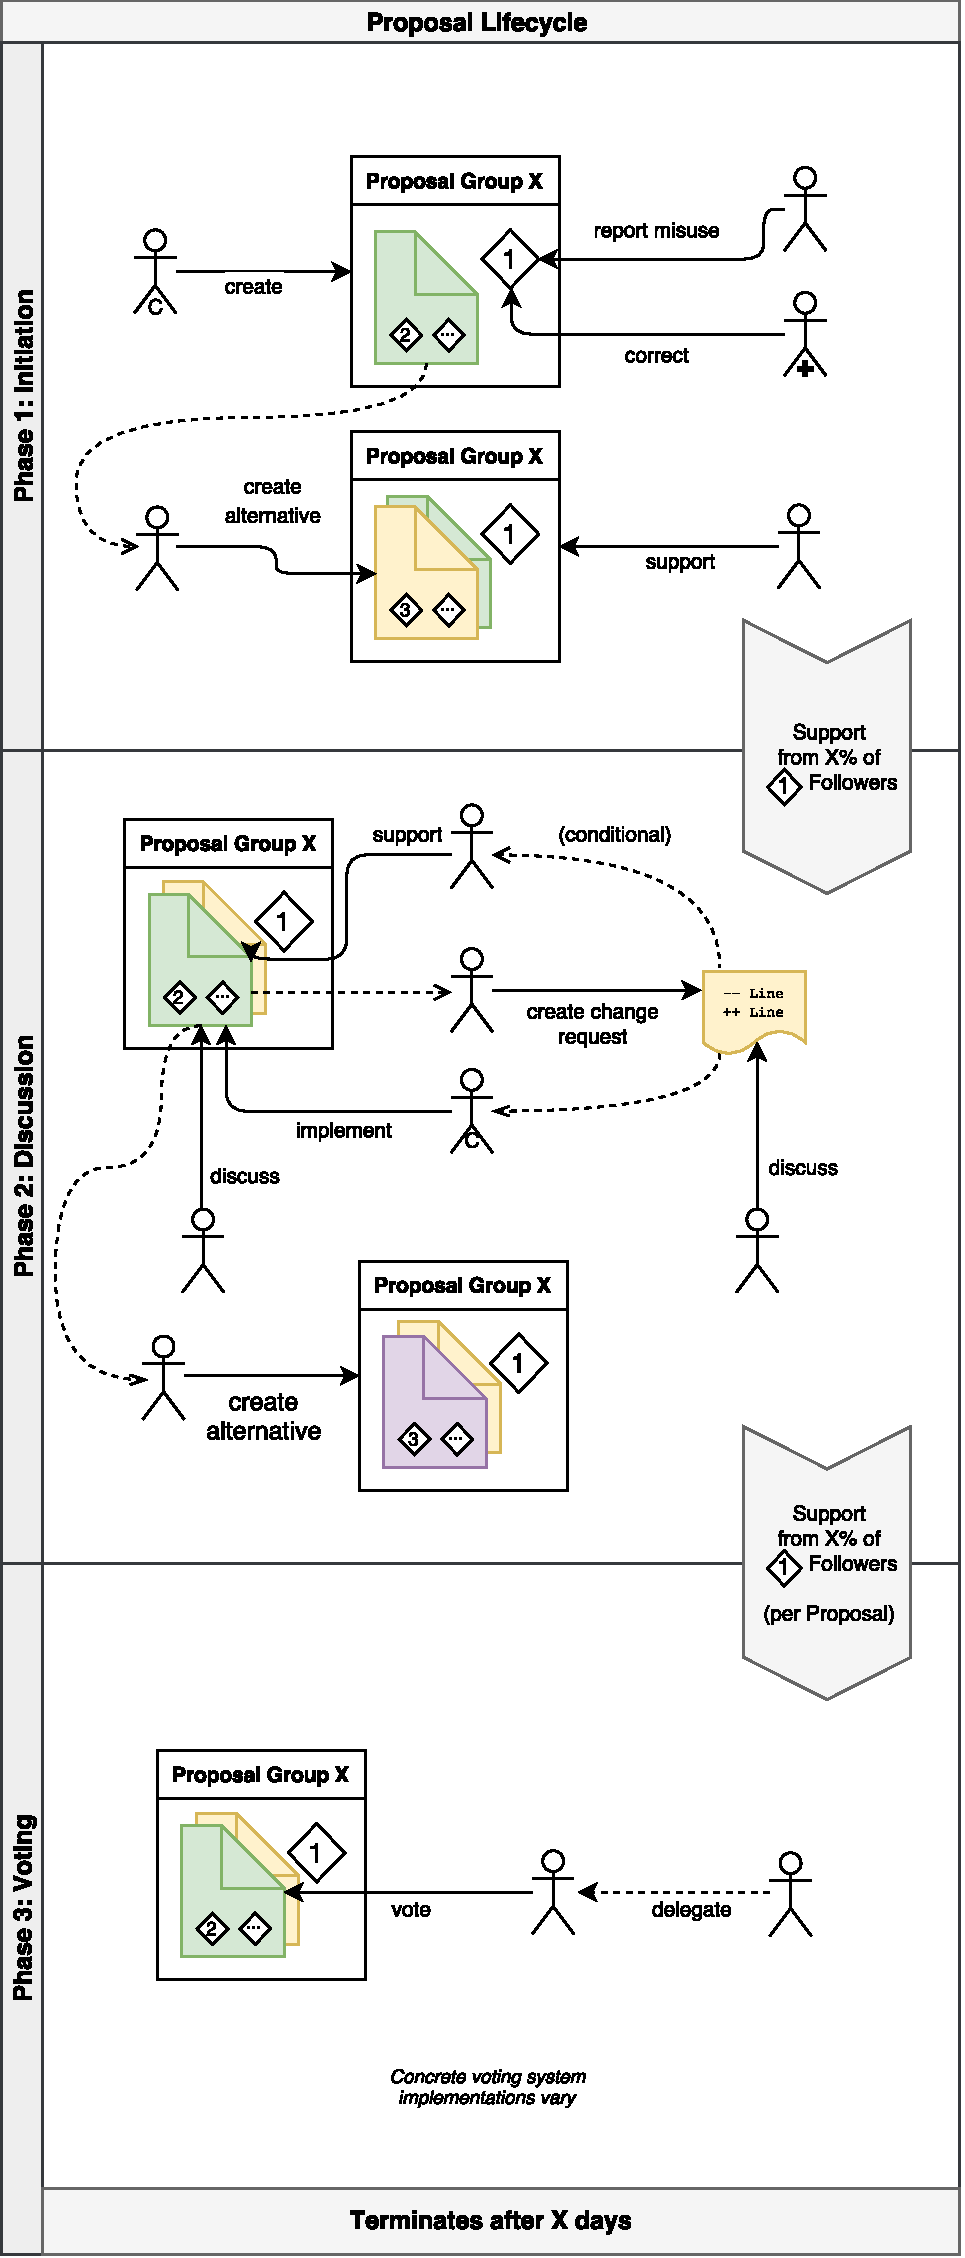
\includegraphics[height=0.6\paperheight]{img/lifecycle_flow_v0.pdf}
\caption{Flow chart of the proposition life cycle}
\label{fig:proplife}
\end{figure}

The life cycle of propositions describes the evolution of a proposition from its initiation to final vote cast.
We split the proposition life cycle into three different phases: (1) initiation, (2) discussion and (3) voting.
It intuitively makes sense to separate a propositions constitutive phase from its voting phase in order to guarantee that the intention of a casted vote stays consistent.
We also subdivide the constitution phase into initiation phase and discussion phase in order to cope with high amounts of individual propositions by allowing only the most appealing propositions to be discussed, thereby channeling the communities efforts and creating an efficient political environment.

In the following, we will successively illustrate each phase by describing its pre- and postconditions as well as its artifacts, actors and their interactions.

\paragraph{Initiation phase}
\label{ssec:Lifecycle_Initiation}

The initiation phase begins when a new proposition is created by a user, which thereby becomes its proposition author (see \ref{ssec:Roles_propositioner}).
To create a proposition, the proposition author needs to specify the following mandatory information: a title, a main text, one primary context, any number of secondary contexts and any number of voting options.
When a new proposition is created, it gets assigned to a new unique proposition group and we call the proposition the \emph{root proposition} of the proposition group.
Other users can then create alternative propositions which share the same proposition group, title and primary context as the root proposition.
Creators of alternative propositions are called alternative proposition authors.
Proposition authors, as well as alternative proposition authors can always edit their respective propositions text, options and secondary contexts.
Followers of a proposition groups primary context that are interested in getting it into the discussion phase can attest their support.
Once a proposition group gains enough support ($X\%$ of the primary context follower population, which $X$ depending on the configuration of the platform implementation), all propositions in it are moved into the discussion phase.

%As the primary context 

\paragraph{Discussion phase}
\label{ssec:Lifecycle_Discussion}

When moving into the discussion phase, more interaction between the supporters and the proposition authors is enabled while all interaction from the initiation phase is maintained.
Users may now issue proposition modification requests to the texts.
Moreover, as previously described in~\ref{ssec:Proposition_Change_Requests}, users can express support for the proposition under the condition that a given modificiation request gets accepted or rejected.
As another means of community involvement in the proposition constitution, users can discuss a proposition.
In discussion entries, special links can be used to reference other artifacts on the platform.
Referencable artifacts are either other discussion entries, (passages of) propositions or (passages of) modification requests.
Other than in the intiation phase, support is not aggregated per proposition group.
Once a single proposition gains enough support ($Y\%$ of the primary context follower population, with $Y$ again depending on the configuration of the platform), it is moved into the voting phase.

\paragraph{Voting phase}
\label{ssec:Lifecycle_Voting}
The voting phase is very different from the two previous phases, as entering it means all abilities to edit the proposition are revoked.
Discussions are still enabled as we do not want to restrict freedom of expression.
With the beginning of the voting phase legitimated users are able to either delegate their vote or place it on their own.
The voting phase ends after a set amount of days that should be specified by the platform admins.
All user intents that are voiced after the voting phase ends are not considered valid.
A detailed description of the voting mechanism is given in the following section.

\subsubsection{User Intent Emission}
\label{sec:User_Intent_Emission}


%Traditionally, in a parliamentarian democracy, the right to initiate and vote on propositions is exclusive for members of the parliament.
%However, in a liquid democracy every citizen has the right to vote on propositions and to participate in their constitutive phase. Consequently, every participant should also have the unrestrained right to create propositions.
%In an anonymized large-scale digital liquid democracy, this right could be abused by malicious users to mass-create spam propositions in order to bury other propositions for example.
%This threat could be tackled by (1) phased proposition life cycles, (2) adaptive sorting algorithms based on bayesian filtering and (3) moderation.
%Moreover, a strategy may involve that a user cannot create more than \textit{n} proposition per month/year.
%The value \textit{n} needs to be carefully chosen, either it is static hard-coded for all citizens or it is dynamically chosen by a citizen’s trustworthiness.

In order for the voting, delegation and supporting mechanisms to fulfill \textbf{(\tracknshrink{LD}2-4)}, they need to be secret, verifiable and decentralized.
Ideally, it shouldn't be possible for any actor in the system to gather any information about a specific users intents, while at the same time being verifiable for any actor that user intents are valid and got counted correctly. 

In line with the principles of security-by-design, in the following we will describe a design for user intent emission that allows manipulation-resistant secret emission of user intents and which largely preserves privacy.
While not being ideal, due to our lack of expertise in zero-knowledge-proof designed systems, the mechanisms described in the following fulfills these criteria well enough for the scope of this work.

The main feature of our system design is that user intents are casted publicly, i.e. they are distributed over the Internet in a way that (1) everyone can access them and (2) no non-critical number of malicious users is able to delete, invalidate or otherwise tamper with user intents.
That means that user intents may be casted using a distributed ledger, a publicly managed collection of mirrored vote servers or any other system that abides by these criteria.

We require one central trusted authority, which (1) distributes \textit{priviledges of participation} amongst authorized users of the platform and (2) provides means of identifying a given user intent as valid.
It thereby contributes to the verifiability of user intents by guaranteeing that valid user intents can only be formulated by authorized individuals, i.e. participants in the platform.
The argument for introducing a centralized service into the system is that in any democratic environment some authority has to decide who is part of that environment and therefore has the right to participate by casting user intents.
Surely, one could imagine a system where the right to vote is granted based on consensus as proposed by the Democracy\.Earth Foundation~\parencite{DemocracyEarth2018}.
However, we do not agree that this system can work on any scale and we are not aware of a way to mathematically prove this assumption.

It is clear that no individual should be able to obtain the privilege of participation multiple times, which can be broken down to the requirements that (R1) no natural person should be able to obtain more than one user accounts and (R2) that no user account should be able to obtain the privilege of participation twice.
Since there is no easy way to solve (R1) purely in the digital realm, it should be the responsibility of the platform operators to come up with a system which distributes unique user accounts to participants without the possibility of malicious persons to obtain more than one.
The second requirement (R2) is easily assured if the trusted authority keeps track of the users which have already obtained their privilege of participation and denies to grant it again.
Note that however this approach is problematic w.r.t. the anonymity property of participation privileges, as the trusted authority could maliciously keep track of which user has been granted which privilege of participation.
However, this problem can be erradicated using a cryptographic method known as blind signature.
By using a blind signature scheme secrecy is preserved because the central authority has no ability to link a given user intent to an identity.
The user intent has been \emph{blindly} singed, and therefore no information about what was signed has been retained. 

In the following we will discuss the interaction of the individual types of user intentions.

\paragraph{Delegation intents}
All the delegation intents of individual users in the same delegation scope implicitly form a delegation graph.
They can be used for all stages of the \hyperref[sec:Model_Propositions]{proposition lifecycle}, i.e. for proposition group initiation support, conditional support in the discussion phase and the voting phase, effectively giving citizen scientists the ability to harvest data about the evolution of the delegation graph from proposition creation to the close of votings.
In order to avoid that changes to more general delegation graphs change the outcome of past votes, delegation intents must be scoped to specific propositions (or proposition groups in the case of support intents in initiation phase).
Note that this does not mean that there can not be context or global scoped delegation graphs in the platform.
Rather, context and global scope delegation graphs could indeed be maintained within the platform.
However, if no delegation intent is issued explicitly by a user, the system would then need to periodically chose the most specific delegation relationship applicable for each user and proposition from these higher level delegation graphs before automatically posting a delegation intent for each combination to the public space.
Although users should be able to change their delegation intents on a given proposition for the entire span of its voting phase, an additional mechanism should ensure that previous delegation intents are invalidated upon issuing a new one.

\paragraph{Vote intents}
As one can easily validate a vote intent against the central trusted authority as well as obtain the power of a vote intent by parsing the delegation graph from the delegation intents in the public space, each individual, even those not involved directly in the platform, has the ability to count and verify votes.
Since users should be able to change their vote intents on a given proposition for the entire span of its voting phase, an additional mechanism should ensure that previous vote intents are invalidated upon issuing a new one.
When building the delegation graph, delegation intents targeted towards a given combination of user and proposition should be invalidated by vote intents targeted towards the same combination, thereby avoiding to count ones vote power twice.

\paragraph{Support intents}
Support intents work just as vote intents, with the following semantical exceptions:
\begin{itemize}
  \item Support intents in the initiation phase are directed towards proposition groups. 
  \item Conditional support intents in the initiation and discussion phase are directed towards proposition change requests.
\end{itemize}






\subsubsection{Vote Counting}
\label{ssec:Vote_Counting}
As we just discussed, our platform design empowers anyone to determine support scores and voting results by parsing delegation, support and vote intents from the public space.
As counting support scores and counting votes have merely semantical differences, for sake of brevity we chose to only describe the vote counting process here:

\begin{enumerate}
  \item For a given proposition $p$, collect all user intents from the public space
  \item Build the delegation graph $\mathcal{D}$ from the delegation intents
  \item Invert all edges in $\mathcal{D}$ to obtain $\mathcal{D}^I$\footnote{Replace all directed edges $(u,v)$ by edges $(v,u)$, $u,v \in N, (u,v) \in E$, with $D=(N,E)$}
  \item All vote intents are collected in a list $V$
  \item If $V$ is not exhausted, assign the next vote intent in $V$ to $v$, else terminate
  \item Check $v$ against the central trusted authority for validity 
  \item If $v$ is not valid, return to number 5
  \item Initialize the voting power $p_v$ of $v$ to 1
  \item If $\mathcal{D}^I$ does not contain $v$, advance to number 13
  \item Remove all incoming edges of $v$ in $\mathcal{D}^I$
  \item Find all nodes $S$ in $\mathcal{D}^I$ that are reachable from $v$
  \item Set $p_v$ to $|S|+1$
  \item In the voting protocol, add $p_v$ to the vote count for the option that $v$ voted for
  \item Return to number 5
\end{enumerate}


\subsubsection{Context Taxonomy Evolution}
\label{ssec:Context_Taxonomy_Evolution}
The evolution of the context taxonomy should be a joint effort between users interested in particular contexts and responsible moderators.
Therefore, the platform should allow for discussions on specific contexts.
Whenever an (informal) consensus is reached among participants in such discussions, responsible moderators should contact the platform admins which can then implement the change.

For reasons of data integrity, changes to the context taxonomy should be very well justified and moderators should in general have rather conservative stances on changing the context taxonomy.

We therefore decided to not design specific artifacts and roles to make this process more automatable and independent from the platform administrators.
Another argument for this non-integrative approach is that, depending on the actual platform implementation, it might not be trivial to guarantee data integrity for specific taxonomy changes and hence might require expert knowledge to execute.


%\subsection{Feedback von Stimmendelegation}
% * <johanning@informatik.uni-leipzig.de> 2018-02-12T12:49:41.623Z:
% 
% > \subsection{Feedback von Stimmendelegation}
% > \label{sec:Model_VoteFeedback}
% > Feedback on the delegation of votes is mediated through notifications. 
% > As mentioned in \ref{sec:Notifications}, delegators are notified when their votes are used in a 'relevant' way by the delegate. Relevancy is managed through user profile settings. 
% 
% What was this supposed to be about (unless I was the one putting it in)?
% 
% ^.
%\label{sec:Model_VoteFeedback}
%Feedback on the delegation of votes is mediated through notifications. 
%As mentioned in \ref{sec:Notifications}, delegators are notified when their votes are used in a 'relevant' way by the delegate. Relevancy is managed through user profile settings. 




\subsubsection{Transparent Data Access}
\label{sec:Model_ResearchersAccess}

As we have argued in \autoref{sec:Criteria} sensitive data of users needs to be protected while still allowing citizen scientists to access information relevant to their specific project.
However, most of the data artifacts we discussed in \autoref{ssec:data_fragments} are not sensitive and could easily be anonymized by replacing references to users with generic hashes in propositions, proposition modification requests and discussion entries.
User accounts could also be opened up to citizen scientists through removing sensitive information such as full name, age and residency from them and additionally providing some binary properties that indicate presence of information in the original data.
We can therefore see that by providing all the non-sensitive information through a well documented interface, we satisfy the requirements of \textbf{(\tracknshrink{CS}1)}.

It could be argued that this approach is too restrictive and unnecessary, since all the data visible on the platform could also be crawled by citizen scientists, but as these probably want to republish some of the data together with their findings and users could withdraw information from the platform in the meantime, citizen scientists should adhere to fair play in this regards in order to not get involved in legal issues.

The most sensitive information in a \tracknshrink{LD} platform, the user intents, are at the same time probably the most interesting and valuable for citizen scientists.
Note that our design of user intents and their emission in the public space as described in \autoref{ssec:User_Intents} and \autoref{sec:User_Intent_Emission} already satisfy the requirements of \textbf{(\tracknshrink{CS}2)}.
They fully preserve privacy, as (1) the original creator of a user intention can not be deduced by the user intent itself and (2) by forcing delegation intents to be reduced to proposition scope, it is possible to generate anonymized user aliases per proposition such that deducing information about single users through structural analysis of multiple delegation graphs is not possible.

The easiest way to solve \textbf{(\tracknshrink{CS}3)} would be to give the user the choice to completely disregard privacy by loosening up all information to citizen scientist access.
However we do not think that a lot of users would choose this option.
A more careful approach is therefore necessary.
Very sensitive personal information such as full name, age and residency should be stripped away regardlessly.
However, the protection from structural analysis could be weakened, such that it would theoretically be possible for adversaries to deduce the political intentions of at least a few users.

This probably less threatening option could be made even safer for users by using techniques as discussed in \autoref{ssec:Integration_pattern}.
Users could opt-in to collect references to user intents they issued together with a proof of ownership.
These references could then be periodically submitted to a server hosted by a trusted citizen science project.
The server could then infer links between multiple delegation graphs and through machine learning synthesize a specialized dataset with similar characteristics relevant to the specific project.
Afterwards, the server would delete the sensitive information and publish the synthetic dataset.

Obviously, this option is only safer w.r.t. users perception, as they need to establish trust towards the operators of a given citizen science project.
This does however not guard against misuse of the sensible informations by either the projects operators themselves or adversaries that could gain access to the server through security breaches and users should be made aware of this when given the option.
Zero-knowledge proofs are outside the scope of this work, but it could be an interesting direction for future research to investigate methods to  cryptographically ensure privacy protection for this data synthesizing 


%% * <johanning@informatik.uni-leipzig.de> 2018-02-12T12:15:14.572Z:
%% 
%% > \subsection{Researchers Access}
%% > \label{sec:Model_ResearchersAccess}
%% 
%% How concrete should we sketch this? Right now its just a 'we need to be aware of this', but I feel it needs to be more concrete...
%% 
%% ^.
%
%
%
%
%While this can't be implemented to its fullest within the scope of this project, this aspect needs considerable consideration in the development of the platform (i.e. in ch. \ref{ch:ProjectRequirements}).
%
%%Steven
%\subsection{Visualization of the Processes}
%\label{sec:Model_Visualization}
%
%%Clara, Simon
%\subsection{Citizen Science Lab Processes}
%\label{sec:CSLab_Processes}
%% Prozess vom Lab schildern, also Fragestellung, Datensammeln, Analysieren und Publizieren: Hier einleiten
%
%%darstellen wie wiss. und nicht-wiss. zusammenarbeiten; inwiefern citizens mÓglichkeit haben in prozess einbezogen zu werden und zu agieren
%
%The workflow of the citizen science lab is sketched in the following.
%
%\subsubsection{Involvement in Formulating Research Questions}
%
%\subsubsection{Citizen Data Collection Process}
%
%\subsubsection{Data Analysis Tools}
%
%\subsubsection{Citizen Science Publication Process}
